% f2_amp.tex -- Figure 2: step 1, from one image to p numbers (natural width about 17.4 cm).
%   (a) the image (plus the small noise) goes through the frozen U-Net of the CIFAR-10 model: 34 blocks drawn one by one with their output
%       size (32x32, 16x16, 8x8; hl_meta.json); block A = the 23rd (dec.16x16_up, red); the 11 blocks after A are not computed (dashed).
%   (b) how one number a_h is read from block h (here the 7th block, enc.16x16_block0: 256 channels of 16x16): steps 1-4 of eq. (2).
%   The channel map is a schematic (gen/mk_data.py), not a real activation.  Colours: navy = block h and its number, red = block A and
%   the largest deviation.
\begin{tikzpicture}[>={Stealth[length=1.8mm, width=1.4mm]}, line cap=round, line join=round, font=\footnotesize,
  lab/.style={inner sep=1pt, align=center, font=\footnotesize}, sm/.style={inner sep=1pt, align=center, font=\scriptsize},
  ttl/.style={anchor=west, inner sep=0pt, font=\small}]
% written by gen/mk_data.py: schematic 16x16 channel map (row-major from the top left); darker = larger
\def\cellsraw{%
\fill[black!23] (0,0) rectangle ++(1,-1);\fill[black!27] (1,0) rectangle ++(1,-1);\fill[black!32] (2,0) rectangle ++(1,-1);\fill[black!37] (3,0) rectangle ++(1,-1);\fill[black!31] (4,0) rectangle ++(1,-1);\fill[black!40] (5,0) rectangle ++(1,-1);\fill[black!25] (6,0) rectangle ++(1,-1);\fill[black!40] (7,0) rectangle ++(1,-1);\fill[black!29] (8,0) rectangle ++(1,-1);\fill[black!27] (9,0) rectangle ++(1,-1);\fill[black!17] (10,0) rectangle ++(1,-1);\fill[black!22] (11,0) rectangle ++(1,-1);\fill[black!14] (12,0) rectangle ++(1,-1);\fill[black!29] (13,0) rectangle ++(1,-1);\fill[black!22] (14,0) rectangle ++(1,-1);\fill[black!24] (15,0) rectangle ++(1,-1);%
\fill[black!15] (0,-1) rectangle ++(1,-1);\fill[black!28] (1,-1) rectangle ++(1,-1);\fill[black!27] (2,-1) rectangle ++(1,-1);\fill[black!48] (3,-1) rectangle ++(1,-1);\fill[black!40] (4,-1) rectangle ++(1,-1);\fill[black!33] (5,-1) rectangle ++(1,-1);\fill[black!35] (6,-1) rectangle ++(1,-1);\fill[black!36] (7,-1) rectangle ++(1,-1);\fill[black!30] (8,-1) rectangle ++(1,-1);\fill[black!22] (9,-1) rectangle ++(1,-1);\fill[black!28] (10,-1) rectangle ++(1,-1);\fill[black!29] (11,-1) rectangle ++(1,-1);\fill[black!14] (12,-1) rectangle ++(1,-1);\fill[black!17] (13,-1) rectangle ++(1,-1);\fill[black!13] (14,-1) rectangle ++(1,-1);\fill[black!16] (15,-1) rectangle ++(1,-1);%
\fill[black!19] (0,-2) rectangle ++(1,-1);\fill[black!30] (1,-2) rectangle ++(1,-1);\fill[black!39] (2,-2) rectangle ++(1,-1);\fill[black!27] (3,-2) rectangle ++(1,-1);\fill[black!36] (4,-2) rectangle ++(1,-1);\fill[black!29] (5,-2) rectangle ++(1,-1);\fill[black!25] (6,-2) rectangle ++(1,-1);\fill[black!35] (7,-2) rectangle ++(1,-1);\fill[black!41] (8,-2) rectangle ++(1,-1);\fill[black!26] (9,-2) rectangle ++(1,-1);\fill[black!24] (10,-2) rectangle ++(1,-1);\fill[black!35] (11,-2) rectangle ++(1,-1);\fill[black!25] (12,-2) rectangle ++(1,-1);\fill[black!29] (13,-2) rectangle ++(1,-1);\fill[black!14] (14,-2) rectangle ++(1,-1);\fill[black!18] (15,-2) rectangle ++(1,-1);%
\fill[black!26] (0,-3) rectangle ++(1,-1);\fill[black!27] (1,-3) rectangle ++(1,-1);\fill[black!20] (2,-3) rectangle ++(1,-1);\fill[black!40] (3,-3) rectangle ++(1,-1);\fill[black!38] (4,-3) rectangle ++(1,-1);\fill[black!33] (5,-3) rectangle ++(1,-1);\fill[black!36] (6,-3) rectangle ++(1,-1);\fill[black!40] (7,-3) rectangle ++(1,-1);\fill[black!21] (8,-3) rectangle ++(1,-1);\fill[black!28] (9,-3) rectangle ++(1,-1);\fill[black!39] (10,-3) rectangle ++(1,-1);\fill[black!58] (11,-3) rectangle ++(1,-1);\fill[black!43] (12,-3) rectangle ++(1,-1);\fill[black!23] (13,-3) rectangle ++(1,-1);\fill[black!24] (14,-3) rectangle ++(1,-1);\fill[black!18] (15,-3) rectangle ++(1,-1);%
\fill[black!24] (0,-4) rectangle ++(1,-1);\fill[black!23] (1,-4) rectangle ++(1,-1);\fill[black!34] (2,-4) rectangle ++(1,-1);\fill[black!31] (3,-4) rectangle ++(1,-1);\fill[black!38] (4,-4) rectangle ++(1,-1);\fill[black!32] (5,-4) rectangle ++(1,-1);\fill[black!38] (6,-4) rectangle ++(1,-1);\fill[black!31] (7,-4) rectangle ++(1,-1);\fill[black!28] (8,-4) rectangle ++(1,-1);\fill[black!39] (9,-4) rectangle ++(1,-1);\fill[black!48] (10,-4) rectangle ++(1,-1);\fill[black!80] (11,-4) rectangle ++(1,-1);\fill[black!52] (12,-4) rectangle ++(1,-1);\fill[black!30] (13,-4) rectangle ++(1,-1);\fill[black!26] (14,-4) rectangle ++(1,-1);\fill[black!22] (15,-4) rectangle ++(1,-1);%
\fill[black!29] (0,-5) rectangle ++(1,-1);\fill[black!36] (1,-5) rectangle ++(1,-1);\fill[black!34] (2,-5) rectangle ++(1,-1);\fill[black!38] (3,-5) rectangle ++(1,-1);\fill[black!37] (4,-5) rectangle ++(1,-1);\fill[black!30] (5,-5) rectangle ++(1,-1);\fill[black!24] (6,-5) rectangle ++(1,-1);\fill[black!28] (7,-5) rectangle ++(1,-1);\fill[black!24] (8,-5) rectangle ++(1,-1);\fill[black!28] (9,-5) rectangle ++(1,-1);\fill[black!48] (10,-5) rectangle ++(1,-1);\fill[black!48] (11,-5) rectangle ++(1,-1);\fill[black!32] (12,-5) rectangle ++(1,-1);\fill[black!24] (13,-5) rectangle ++(1,-1);\fill[black!16] (14,-5) rectangle ++(1,-1);\fill[black!25] (15,-5) rectangle ++(1,-1);%
\fill[black!26] (0,-6) rectangle ++(1,-1);\fill[black!19] (1,-6) rectangle ++(1,-1);\fill[black!23] (2,-6) rectangle ++(1,-1);\fill[black!28] (3,-6) rectangle ++(1,-1);\fill[black!16] (4,-6) rectangle ++(1,-1);\fill[black!28] (5,-6) rectangle ++(1,-1);\fill[black!32] (6,-6) rectangle ++(1,-1);\fill[black!37] (7,-6) rectangle ++(1,-1);\fill[black!25] (8,-6) rectangle ++(1,-1);\fill[black!33] (9,-6) rectangle ++(1,-1);\fill[black!28] (10,-6) rectangle ++(1,-1);\fill[black!28] (11,-6) rectangle ++(1,-1);\fill[black!23] (12,-6) rectangle ++(1,-1);\fill[black!26] (13,-6) rectangle ++(1,-1);\fill[black!25] (14,-6) rectangle ++(1,-1);\fill[black!17] (15,-6) rectangle ++(1,-1);%
\fill[black!40] (0,-7) rectangle ++(1,-1);\fill[black!32] (1,-7) rectangle ++(1,-1);\fill[black!21] (2,-7) rectangle ++(1,-1);\fill[black!14] (3,-7) rectangle ++(1,-1);\fill[black!24] (4,-7) rectangle ++(1,-1);\fill[black!22] (5,-7) rectangle ++(1,-1);\fill[black!32] (6,-7) rectangle ++(1,-1);\fill[black!26] (7,-7) rectangle ++(1,-1);\fill[black!23] (8,-7) rectangle ++(1,-1);\fill[black!20] (9,-7) rectangle ++(1,-1);\fill[black!28] (10,-7) rectangle ++(1,-1);\fill[black!23] (11,-7) rectangle ++(1,-1);\fill[black!32] (12,-7) rectangle ++(1,-1);\fill[black!29] (13,-7) rectangle ++(1,-1);\fill[black!24] (14,-7) rectangle ++(1,-1);\fill[black!27] (15,-7) rectangle ++(1,-1);%
\fill[black!24] (0,-8) rectangle ++(1,-1);\fill[black!24] (1,-8) rectangle ++(1,-1);\fill[black!12] (2,-8) rectangle ++(1,-1);\fill[black!19] (3,-8) rectangle ++(1,-1);\fill[black!32] (4,-8) rectangle ++(1,-1);\fill[black!29] (5,-8) rectangle ++(1,-1);\fill[black!36] (6,-8) rectangle ++(1,-1);\fill[black!23] (7,-8) rectangle ++(1,-1);\fill[black!21] (8,-8) rectangle ++(1,-1);\fill[black!33] (9,-8) rectangle ++(1,-1);\fill[black!36] (10,-8) rectangle ++(1,-1);\fill[black!31] (11,-8) rectangle ++(1,-1);\fill[black!46] (12,-8) rectangle ++(1,-1);\fill[black!20] (13,-8) rectangle ++(1,-1);\fill[black!37] (14,-8) rectangle ++(1,-1);\fill[black!36] (15,-8) rectangle ++(1,-1);%
\fill[black!19] (0,-9) rectangle ++(1,-1);\fill[black!33] (1,-9) rectangle ++(1,-1);\fill[black!26] (2,-9) rectangle ++(1,-1);\fill[black!35] (3,-9) rectangle ++(1,-1);\fill[black!17] (4,-9) rectangle ++(1,-1);\fill[black!21] (5,-9) rectangle ++(1,-1);\fill[black!11] (6,-9) rectangle ++(1,-1);\fill[black!30] (7,-9) rectangle ++(1,-1);\fill[black!21] (8,-9) rectangle ++(1,-1);\fill[black!33] (9,-9) rectangle ++(1,-1);\fill[black!15] (10,-9) rectangle ++(1,-1);\fill[black!27] (11,-9) rectangle ++(1,-1);\fill[black!41] (12,-9) rectangle ++(1,-1);\fill[black!35] (13,-9) rectangle ++(1,-1);\fill[black!30] (14,-9) rectangle ++(1,-1);\fill[black!44] (15,-9) rectangle ++(1,-1);%
\fill[black!22] (0,-10) rectangle ++(1,-1);\fill[black!24] (1,-10) rectangle ++(1,-1);\fill[black!24] (2,-10) rectangle ++(1,-1);\fill[black!24] (3,-10) rectangle ++(1,-1);\fill[black!15] (4,-10) rectangle ++(1,-1);\fill[black!30] (5,-10) rectangle ++(1,-1);\fill[black!16] (6,-10) rectangle ++(1,-1);\fill[black!13] (7,-10) rectangle ++(1,-1);\fill[black!24] (8,-10) rectangle ++(1,-1);\fill[black!13] (9,-10) rectangle ++(1,-1);\fill[black!35] (10,-10) rectangle ++(1,-1);\fill[black!35] (11,-10) rectangle ++(1,-1);\fill[black!38] (12,-10) rectangle ++(1,-1);\fill[black!40] (13,-10) rectangle ++(1,-1);\fill[black!41] (14,-10) rectangle ++(1,-1);\fill[black!37] (15,-10) rectangle ++(1,-1);%
\fill[black!19] (0,-11) rectangle ++(1,-1);\fill[black!24] (1,-11) rectangle ++(1,-1);\fill[black!31] (2,-11) rectangle ++(1,-1);\fill[black!18] (3,-11) rectangle ++(1,-1);\fill[black!26] (4,-11) rectangle ++(1,-1);\fill[black!10] (5,-11) rectangle ++(1,-1);\fill[black!21] (6,-11) rectangle ++(1,-1);\fill[black!32] (7,-11) rectangle ++(1,-1);\fill[black!34] (8,-11) rectangle ++(1,-1);\fill[black!22] (9,-11) rectangle ++(1,-1);\fill[black!34] (10,-11) rectangle ++(1,-1);\fill[black!32] (11,-11) rectangle ++(1,-1);\fill[black!31] (12,-11) rectangle ++(1,-1);\fill[black!33] (13,-11) rectangle ++(1,-1);\fill[black!40] (14,-11) rectangle ++(1,-1);\fill[black!39] (15,-11) rectangle ++(1,-1);%
\fill[black!28] (0,-12) rectangle ++(1,-1);\fill[black!23] (1,-12) rectangle ++(1,-1);\fill[black!23] (2,-12) rectangle ++(1,-1);\fill[black!20] (3,-12) rectangle ++(1,-1);\fill[black!14] (4,-12) rectangle ++(1,-1);\fill[black!18] (5,-12) rectangle ++(1,-1);\fill[black!29] (6,-12) rectangle ++(1,-1);\fill[black!19] (7,-12) rectangle ++(1,-1);\fill[black!20] (8,-12) rectangle ++(1,-1);\fill[black!18] (9,-12) rectangle ++(1,-1);\fill[black!25] (10,-12) rectangle ++(1,-1);\fill[black!26] (11,-12) rectangle ++(1,-1);\fill[black!39] (12,-12) rectangle ++(1,-1);\fill[black!32] (13,-12) rectangle ++(1,-1);\fill[black!37] (14,-12) rectangle ++(1,-1);\fill[black!28] (15,-12) rectangle ++(1,-1);%
\fill[black!28] (0,-13) rectangle ++(1,-1);\fill[black!17] (1,-13) rectangle ++(1,-1);\fill[black!22] (2,-13) rectangle ++(1,-1);\fill[black!20] (3,-13) rectangle ++(1,-1);\fill[black!23] (4,-13) rectangle ++(1,-1);\fill[black!11] (5,-13) rectangle ++(1,-1);\fill[black!12] (6,-13) rectangle ++(1,-1);\fill[black!8] (7,-13) rectangle ++(1,-1);\fill[black!13] (8,-13) rectangle ++(1,-1);\fill[black!28] (9,-13) rectangle ++(1,-1);\fill[black!41] (10,-13) rectangle ++(1,-1);\fill[black!31] (11,-13) rectangle ++(1,-1);\fill[black!15] (12,-13) rectangle ++(1,-1);\fill[black!39] (13,-13) rectangle ++(1,-1);\fill[black!34] (14,-13) rectangle ++(1,-1);\fill[black!41] (15,-13) rectangle ++(1,-1);%
\fill[black!37] (0,-14) rectangle ++(1,-1);\fill[black!20] (1,-14) rectangle ++(1,-1);\fill[black!19] (2,-14) rectangle ++(1,-1);\fill[black!14] (3,-14) rectangle ++(1,-1);\fill[black!24] (4,-14) rectangle ++(1,-1);\fill[black!16] (5,-14) rectangle ++(1,-1);\fill[black!18] (6,-14) rectangle ++(1,-1);\fill[black!19] (7,-14) rectangle ++(1,-1);\fill[black!22] (8,-14) rectangle ++(1,-1);\fill[black!23] (9,-14) rectangle ++(1,-1);\fill[black!39] (10,-14) rectangle ++(1,-1);\fill[black!37] (11,-14) rectangle ++(1,-1);\fill[black!35] (12,-14) rectangle ++(1,-1);\fill[black!37] (13,-14) rectangle ++(1,-1);\fill[black!49] (14,-14) rectangle ++(1,-1);\fill[black!47] (15,-14) rectangle ++(1,-1);%
\fill[black!23] (0,-15) rectangle ++(1,-1);\fill[black!18] (1,-15) rectangle ++(1,-1);\fill[black!28] (2,-15) rectangle ++(1,-1);\fill[black!20] (3,-15) rectangle ++(1,-1);\fill[black!19] (4,-15) rectangle ++(1,-1);\fill[black!25] (5,-15) rectangle ++(1,-1);\fill[black!17] (6,-15) rectangle ++(1,-1);\fill[black!17] (7,-15) rectangle ++(1,-1);\fill[black!25] (8,-15) rectangle ++(1,-1);\fill[black!35] (9,-15) rectangle ++(1,-1);\fill[black!26] (10,-15) rectangle ++(1,-1);\fill[black!22] (11,-15) rectangle ++(1,-1);\fill[black!34] (12,-15) rectangle ++(1,-1);\fill[black!42] (13,-15) rectangle ++(1,-1);\fill[black!41] (14,-15) rectangle ++(1,-1);\fill[black!38] (15,-15) rectangle ++(1,-1);%
}
\def\cellsdev{%
\fill[black!15] (0,0) rectangle ++(1,-1);\fill[black!10] (1,0) rectangle ++(1,-1);\fill[black!13] (2,0) rectangle ++(1,-1);\fill[black!20] (3,0) rectangle ++(1,-1);\fill[black!12] (4,0) rectangle ++(1,-1);\fill[black!25] (5,0) rectangle ++(1,-1);\fill[black!12] (6,0) rectangle ++(1,-1);\fill[black!24] (7,0) rectangle ++(1,-1);\fill[black!9] (8,0) rectangle ++(1,-1);\fill[black!10] (9,0) rectangle ++(1,-1);\fill[black!24] (10,0) rectangle ++(1,-1);\fill[black!16] (11,0) rectangle ++(1,-1);\fill[black!27] (12,0) rectangle ++(1,-1);\fill[black!9] (13,0) rectangle ++(1,-1);\fill[black!16] (14,0) rectangle ++(1,-1);\fill[black!14] (15,0) rectangle ++(1,-1);%
\fill[black!26] (0,-1) rectangle ++(1,-1);\fill[black!8] (1,-1) rectangle ++(1,-1);\fill[black!9] (2,-1) rectangle ++(1,-1);\fill[black!36] (3,-1) rectangle ++(1,-1);\fill[black!24] (4,-1) rectangle ++(1,-1);\fill[black!15] (5,-1) rectangle ++(1,-1);\fill[black!17] (6,-1) rectangle ++(1,-1);\fill[black!19] (7,-1) rectangle ++(1,-1);\fill[black!11] (8,-1) rectangle ++(1,-1);\fill[black!17] (9,-1) rectangle ++(1,-1);\fill[black!9] (10,-1) rectangle ++(1,-1);\fill[black!9] (11,-1) rectangle ++(1,-1);\fill[black!27] (12,-1) rectangle ++(1,-1);\fill[black!24] (13,-1) rectangle ++(1,-1);\fill[black!29] (14,-1) rectangle ++(1,-1);\fill[black!24] (15,-1) rectangle ++(1,-1);%
\fill[black!20] (0,-2) rectangle ++(1,-1);\fill[black!11] (1,-2) rectangle ++(1,-1);\fill[black!23] (2,-2) rectangle ++(1,-1);\fill[black!10] (3,-2) rectangle ++(1,-1);\fill[black!19] (4,-2) rectangle ++(1,-1);\fill[black!9] (5,-2) rectangle ++(1,-1);\fill[black!12] (6,-2) rectangle ++(1,-1);\fill[black!18] (7,-2) rectangle ++(1,-1);\fill[black!27] (8,-2) rectangle ++(1,-1);\fill[black!11] (9,-2) rectangle ++(1,-1);\fill[black!14] (10,-2) rectangle ++(1,-1);\fill[black!17] (11,-2) rectangle ++(1,-1);\fill[black!12] (12,-2) rectangle ++(1,-1);\fill[black!9] (13,-2) rectangle ++(1,-1);\fill[black!28] (14,-2) rectangle ++(1,-1);\fill[black!22] (15,-2) rectangle ++(1,-1);%
\fill[black!11] (0,-3) rectangle ++(1,-1);\fill[black!9] (1,-3) rectangle ++(1,-1);\fill[black!19] (2,-3) rectangle ++(1,-1);\fill[black!24] (3,-3) rectangle ++(1,-1);\fill[black!21] (4,-3) rectangle ++(1,-1);\fill[black!14] (5,-3) rectangle ++(1,-1);\fill[black!19] (6,-3) rectangle ++(1,-1);\fill[black!24] (7,-3) rectangle ++(1,-1);\fill[black!18] (8,-3) rectangle ++(1,-1);\fill[black!8] (9,-3) rectangle ++(1,-1);\fill[black!23] (10,-3) rectangle ++(1,-1);\fill[black!50] (11,-3) rectangle ++(1,-1);\fill[black!29] (12,-3) rectangle ++(1,-1);\fill[black!14] (13,-3) rectangle ++(1,-1);\fill[black!13] (14,-3) rectangle ++(1,-1);\fill[black!22] (15,-3) rectangle ++(1,-1);%
\fill[black!13] (0,-4) rectangle ++(1,-1);\fill[black!16] (1,-4) rectangle ++(1,-1);\fill[black!17] (2,-4) rectangle ++(1,-1);\fill[black!12] (3,-4) rectangle ++(1,-1);\fill[black!22] (4,-4) rectangle ++(1,-1);\fill[black!14] (5,-4) rectangle ++(1,-1);\fill[black!21] (6,-4) rectangle ++(1,-1);\fill[black!12] (7,-4) rectangle ++(1,-1);\fill[black!8] (8,-4) rectangle ++(1,-1);\fill[black!23] (9,-4) rectangle ++(1,-1);\fill[black!36] (10,-4) rectangle ++(1,-1);\fill[black!80] (11,-4) rectangle ++(1,-1);\fill[black!42] (12,-4) rectangle ++(1,-1);\fill[black!11] (13,-4) rectangle ++(1,-1);\fill[black!11] (14,-4) rectangle ++(1,-1);\fill[black!16] (15,-4) rectangle ++(1,-1);%
\fill[black!9] (0,-5) rectangle ++(1,-1);\fill[black!20] (1,-5) rectangle ++(1,-1);\fill[black!17] (2,-5) rectangle ++(1,-1);\fill[black!22] (3,-5) rectangle ++(1,-1);\fill[black!20] (4,-5) rectangle ++(1,-1);\fill[black!11] (5,-5) rectangle ++(1,-1);\fill[black!14] (6,-5) rectangle ++(1,-1);\fill[black!8] (7,-5) rectangle ++(1,-1);\fill[black!14] (8,-5) rectangle ++(1,-1);\fill[black!8] (9,-5) rectangle ++(1,-1);\fill[black!35] (10,-5) rectangle ++(1,-1);\fill[black!35] (11,-5) rectangle ++(1,-1);\fill[black!14] (12,-5) rectangle ++(1,-1);\fill[black!14] (13,-5) rectangle ++(1,-1);\fill[black!25] (14,-5) rectangle ++(1,-1);\fill[black!12] (15,-5) rectangle ++(1,-1);%
\fill[black!11] (0,-6) rectangle ++(1,-1);\fill[black!20] (1,-6) rectangle ++(1,-1);\fill[black!16] (2,-6) rectangle ++(1,-1);\fill[black!9] (3,-6) rectangle ++(1,-1);\fill[black!24] (4,-6) rectangle ++(1,-1);\fill[black!8] (5,-6) rectangle ++(1,-1);\fill[black!13] (6,-6) rectangle ++(1,-1);\fill[black!21] (7,-6) rectangle ++(1,-1);\fill[black!13] (8,-6) rectangle ++(1,-1);\fill[black!15] (9,-6) rectangle ++(1,-1);\fill[black!8] (10,-6) rectangle ++(1,-1);\fill[black!8] (11,-6) rectangle ++(1,-1);\fill[black!15] (12,-6) rectangle ++(1,-1);\fill[black!11] (13,-6) rectangle ++(1,-1);\fill[black!12] (14,-6) rectangle ++(1,-1);\fill[black!24] (15,-6) rectangle ++(1,-1);%
\fill[black!24] (0,-7) rectangle ++(1,-1);\fill[black!13] (1,-7) rectangle ++(1,-1);\fill[black!17] (2,-7) rectangle ++(1,-1);\fill[black!28] (3,-7) rectangle ++(1,-1);\fill[black!14] (4,-7) rectangle ++(1,-1);\fill[black!16] (5,-7) rectangle ++(1,-1);\fill[black!14] (6,-7) rectangle ++(1,-1);\fill[black!11] (7,-7) rectangle ++(1,-1);\fill[black!16] (8,-7) rectangle ++(1,-1);\fill[black!19] (9,-7) rectangle ++(1,-1);\fill[black!8] (10,-7) rectangle ++(1,-1);\fill[black!15] (11,-7) rectangle ++(1,-1);\fill[black!14] (12,-7) rectangle ++(1,-1);\fill[black!10] (13,-7) rectangle ++(1,-1);\fill[black!14] (14,-7) rectangle ++(1,-1);\fill[black!9] (15,-7) rectangle ++(1,-1);%
\fill[black!14] (0,-8) rectangle ++(1,-1);\fill[black!14] (1,-8) rectangle ++(1,-1);\fill[black!31] (2,-8) rectangle ++(1,-1);\fill[black!20] (3,-8) rectangle ++(1,-1);\fill[black!14] (4,-8) rectangle ++(1,-1);\fill[black!9] (5,-8) rectangle ++(1,-1);\fill[black!19] (6,-8) rectangle ++(1,-1);\fill[black!15] (7,-8) rectangle ++(1,-1);\fill[black!17] (8,-8) rectangle ++(1,-1);\fill[black!15] (9,-8) rectangle ++(1,-1);\fill[black!19] (10,-8) rectangle ++(1,-1);\fill[black!12] (11,-8) rectangle ++(1,-1);\fill[black!32] (12,-8) rectangle ++(1,-1);\fill[black!19] (13,-8) rectangle ++(1,-1);\fill[black!20] (14,-8) rectangle ++(1,-1);\fill[black!19] (15,-8) rectangle ++(1,-1);%
\fill[black!21] (0,-9) rectangle ++(1,-1);\fill[black!15] (1,-9) rectangle ++(1,-1);\fill[black!11] (2,-9) rectangle ++(1,-1);\fill[black!18] (3,-9) rectangle ++(1,-1);\fill[black!23] (4,-9) rectangle ++(1,-1);\fill[black!18] (5,-9) rectangle ++(1,-1);\fill[black!31] (6,-9) rectangle ++(1,-1);\fill[black!10] (7,-9) rectangle ++(1,-1);\fill[black!17] (8,-9) rectangle ++(1,-1);\fill[black!15] (9,-9) rectangle ++(1,-1);\fill[black!26] (10,-9) rectangle ++(1,-1);\fill[black!10] (11,-9) rectangle ++(1,-1);\fill[black!25] (12,-9) rectangle ++(1,-1);\fill[black!18] (13,-9) rectangle ++(1,-1);\fill[black!10] (14,-9) rectangle ++(1,-1);\fill[black!30] (15,-9) rectangle ++(1,-1);%
\fill[black!17] (0,-10) rectangle ++(1,-1);\fill[black!14] (1,-10) rectangle ++(1,-1);\fill[black!13] (2,-10) rectangle ++(1,-1);\fill[black!14] (3,-10) rectangle ++(1,-1);\fill[black!26] (4,-10) rectangle ++(1,-1);\fill[black!11] (5,-10) rectangle ++(1,-1);\fill[black!25] (6,-10) rectangle ++(1,-1);\fill[black!30] (7,-10) rectangle ++(1,-1);\fill[black!13] (8,-10) rectangle ++(1,-1);\fill[black!29] (9,-10) rectangle ++(1,-1);\fill[black!17] (10,-10) rectangle ++(1,-1);\fill[black!18] (11,-10) rectangle ++(1,-1);\fill[black!22] (12,-10) rectangle ++(1,-1);\fill[black!24] (13,-10) rectangle ++(1,-1);\fill[black!26] (14,-10) rectangle ++(1,-1);\fill[black!21] (15,-10) rectangle ++(1,-1);%
\fill[black!20] (0,-11) rectangle ++(1,-1);\fill[black!14] (1,-11) rectangle ++(1,-1);\fill[black!12] (2,-11) rectangle ++(1,-1);\fill[black!22] (3,-11) rectangle ++(1,-1);\fill[black!11] (4,-11) rectangle ++(1,-1);\fill[black!33] (5,-11) rectangle ++(1,-1);\fill[black!17] (6,-11) rectangle ++(1,-1);\fill[black!14] (7,-11) rectangle ++(1,-1);\fill[black!16] (8,-11) rectangle ++(1,-1);\fill[black!17] (9,-11) rectangle ++(1,-1);\fill[black!16] (10,-11) rectangle ++(1,-1);\fill[black!13] (11,-11) rectangle ++(1,-1);\fill[black!13] (12,-11) rectangle ++(1,-1);\fill[black!15] (13,-11) rectangle ++(1,-1);\fill[black!25] (14,-11) rectangle ++(1,-1);\fill[black!23] (15,-11) rectangle ++(1,-1);%
\fill[black!8] (0,-12) rectangle ++(1,-1);\fill[black!15] (1,-12) rectangle ++(1,-1);\fill[black!15] (2,-12) rectangle ++(1,-1);\fill[black!19] (3,-12) rectangle ++(1,-1);\fill[black!27] (4,-12) rectangle ++(1,-1);\fill[black!22] (5,-12) rectangle ++(1,-1);\fill[black!10] (6,-12) rectangle ++(1,-1);\fill[black!21] (7,-12) rectangle ++(1,-1);\fill[black!20] (8,-12) rectangle ++(1,-1);\fill[black!23] (9,-12) rectangle ++(1,-1);\fill[black!12] (10,-12) rectangle ++(1,-1);\fill[black!10] (11,-12) rectangle ++(1,-1);\fill[black!24] (12,-12) rectangle ++(1,-1);\fill[black!14] (13,-12) rectangle ++(1,-1);\fill[black!20] (14,-12) rectangle ++(1,-1);\fill[black!8] (15,-12) rectangle ++(1,-1);%
\fill[black!9] (0,-13) rectangle ++(1,-1);\fill[black!24] (1,-13) rectangle ++(1,-1);\fill[black!17] (2,-13) rectangle ++(1,-1);\fill[black!19] (3,-13) rectangle ++(1,-1);\fill[black!15] (4,-13) rectangle ++(1,-1);\fill[black!32] (5,-13) rectangle ++(1,-1);\fill[black!31] (6,-13) rectangle ++(1,-1);\fill[black!36] (7,-13) rectangle ++(1,-1);\fill[black!29] (8,-13) rectangle ++(1,-1);\fill[black!9] (9,-13) rectangle ++(1,-1);\fill[black!25] (10,-13) rectangle ++(1,-1);\fill[black!12] (11,-13) rectangle ++(1,-1);\fill[black!27] (12,-13) rectangle ++(1,-1);\fill[black!23] (13,-13) rectangle ++(1,-1);\fill[black!17] (14,-13) rectangle ++(1,-1);\fill[black!26] (15,-13) rectangle ++(1,-1);%
\fill[black!21] (0,-14) rectangle ++(1,-1);\fill[black!19] (1,-14) rectangle ++(1,-1);\fill[black!21] (2,-14) rectangle ++(1,-1);\fill[black!27] (3,-14) rectangle ++(1,-1);\fill[black!13] (4,-14) rectangle ++(1,-1);\fill[black!25] (5,-14) rectangle ++(1,-1);\fill[black!22] (6,-14) rectangle ++(1,-1);\fill[black!21] (7,-14) rectangle ++(1,-1);\fill[black!16] (8,-14) rectangle ++(1,-1);\fill[black!16] (9,-14) rectangle ++(1,-1);\fill[black!23] (10,-14) rectangle ++(1,-1);\fill[black!21] (11,-14) rectangle ++(1,-1);\fill[black!17] (12,-14) rectangle ++(1,-1);\fill[black!20] (13,-14) rectangle ++(1,-1);\fill[black!38] (14,-14) rectangle ++(1,-1);\fill[black!35] (15,-14) rectangle ++(1,-1);%
\fill[black!15] (0,-15) rectangle ++(1,-1);\fill[black!22] (1,-15) rectangle ++(1,-1);\fill[black!8] (2,-15) rectangle ++(1,-1);\fill[black!19] (3,-15) rectangle ++(1,-1);\fill[black!21] (4,-15) rectangle ++(1,-1);\fill[black!12] (5,-15) rectangle ++(1,-1);\fill[black!24] (6,-15) rectangle ++(1,-1);\fill[black!24] (7,-15) rectangle ++(1,-1);\fill[black!12] (8,-15) rectangle ++(1,-1);\fill[black!17] (9,-15) rectangle ++(1,-1);\fill[black!10] (10,-15) rectangle ++(1,-1);\fill[black!17] (11,-15) rectangle ++(1,-1);\fill[black!17] (12,-15) rectangle ++(1,-1);\fill[black!27] (13,-15) rectangle ++(1,-1);\fill[black!26] (14,-15) rectangle ++(1,-1);\fill[black!21] (15,-15) rectangle ++(1,-1);%
}
\def\cellmaxrow{4}\def\cellmaxcol{11}

% ================================================================ (a)
\node[ttl] at (0,0.3) {\textbf{(a)}\ 画像を通し,ブロックごとに数を1つ読む};
\node[inner sep=0, draw=black!60] (im) at (0.75,-1.25) {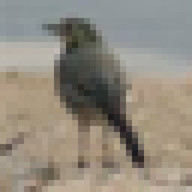
\includegraphics[width=1.25cm]{img/b_o0.png}};
\node[lab, anchor=north] at (0.75,-1.95) {画像 $\vec{x}$};
\node[sm, anchor=north, text=black!70] at (0.75,-2.33) {$3{\times}32{\times}32$ 個の数};
\draw[->] (1.45,-1.25) -- node[above, lab] {$+\sigma_{1}\vec{\varepsilon}$} (2.3,-1.25);
% the 34 blocks: resolution of the output 32, 16, 8 (height 1.5, 1.0, 0.6 cm)
\def\blk#1#2#3{% index, resolution, style
  \pgfmathsetmacro{\bx}{2.45+(#1-1)*0.17}
  \ifnum#2=32 \def\bh{1.5}\def\bc{-1.0}\fi
  \ifnum#2=16 \def\bh{1.0}\def\bc{-1.4}\fi
  \ifnum#2=8 \def\bh{0.6}\def\bc{-1.75}\fi
  \draw[#3] (\bx,\bc-\bh/2) rectangle ++(0.11,\bh);}
\foreach \i/\r in {1/32,2/32,3/32,4/32,5/32,6/16,8/16,9/16,10/16,11/8,12/8,13/8,14/8,15/8,16/8,17/8,18/8,19/8,20/8,21/8,22/8}
  {\blk{\i}{\r}{black, line width=0.45pt}}
\blk{7}{16}{navyc, line width=1.1pt}
\blk{23}{16}{redc, line width=1.1pt}
\foreach \i/\r in {24/16,25/16,26/16,27/16,28/16,29/32,30/32,31/32,32/32,33/32,34/32}
  {\blk{\i}{\r}{black!35, densely dashed, line width=0.4pt}}
\node[lab, anchor=south] at (5.31,-0.2) {U-Net(凍結)\ \ ブロックは34個};
\node[lab, text=navyc, anchor=south] at (3.53,-0.86) {$h$};
\node[lab, text=redc, anchor=south east] at (6.36,-0.86) {(ここで止める)A};
\node[sm, text=black!50, anchor=north] at (7.25,-2.0) {使わない};
\draw[decorate, decoration={brace, mirror, amplitude=3pt}] (2.45,-2.38) -- (6.30,-2.38);
\node[lab, anchor=north] at (4.38,-2.5) {ブロック1〜A ($p=23$ 個)};
\draw[->] (8.45,-0.75) -- (16.05,-0.75);
\node[lab, anchor=south] at (12.2,-0.7) {ブロック1〜Aのそれぞれから数を1つ\\(振幅 $a_{h}$)読み,縦に並べる};
\node[lab, anchor=north, text=black!70] at (12.2,-0.82) {1つの数の読み方は(b)};
% ---- the profile: p x 1, cells of 0.19 cm
\begin{scope}[shift={(16.15,-0.15)}]
  \foreach \k in {1,...,23} \draw[black, line width=0.4pt] (0,{-(\k-1)*0.19}) rectangle ++(0.3,-0.19);
  \draw[navyc, line width=1.1pt] (0,{-6*0.19}) rectangle ++(0.3,-0.19);
  \draw[redc, line width=1.1pt] (0,{-22*0.19}) rectangle ++(0.3,-0.19);
  \node[sm, anchor=west] at (0.33,-0.095) {$a_{1}$};
  \node[sm, anchor=west, text=navyc] at (0.33,{-6.5*0.19}) {$a_{h}$};
  \node[sm, anchor=west, text=redc] at (0.33,{-22.5*0.19}) {$a_{p}$(A)};
  \node[lab, anchor=south] at (0.15,0.02) {$\vec{a}(\vec{x})$};
  \node[sm, anchor=north] at (0.15,-4.43) {$p{\times}1$};
\end{scope}
% ================================================================ (b)
\begin{scope}[shift={(0,-0.2)}]
\node[ttl] at (0,-3.0) {\textbf{(b)}\ ブロック $h$(紺. 図では7番目)の出力から数を1つ読む(式~\eqref{eq:amp}の\cn{1}〜\cn{4})};
% stack of the C_h channel maps
\foreach \s in {4,3,2,1,0} \draw[black, line width=0.45pt, fill=white] ({0.25+0.1*\s},{-3.35-0.1*\s}) rectangle ++(1.25,-1.25);
\node[sm, anchor=north] at (1.15,-5.12) {$C_{h}=256$ 枚};
\node[sm, anchor=north] at (1.15,-5.45) {(チャネル $j$)};
\draw[->] (2.05,-4.15) -- node[above, sm] {$j$ 枚目} (2.65,-4.15);
% one channel: 16 x 16 values (cell 0.1 cm)
\begin{scope}[shift={(2.75,-3.35)}, x=0.1cm, y=0.1cm]
  \cellsraw
  \draw[black, line width=0.45pt] (0,0) rectangle (16,-16);
\end{scope}
\node[sm, anchor=north] at (3.55,-5.0) {$U_{h}=16{\times}16$ 個の値};
\node[sm, anchor=north] at (3.55,-5.33) {$f_{h,j,u}(\vec{x})$};
\draw[->] (4.45,-4.15) -- (6.15,-4.15);
\node[sm, anchor=south] at (5.3,-4.08) {\cn{1}\,平均を引く};
\node[sm, anchor=north] at (5.3,-4.22) {\cn{2}\,絶対値};
% |f - mean|: the largest one in red
\begin{scope}[shift={(6.25,-3.35)}, x=0.1cm, y=0.1cm]
  \cellsdev
  \draw[black, line width=0.45pt] (0,0) rectangle (16,-16);
  \draw[redc, line width=1.0pt] (\cellmaxcol,-\cellmaxrow) rectangle ++(1,-1);
\end{scope}
\node[sm, anchor=north] at (7.05,-5.0) {$|f_{h,j,u}(\vec{x})-\bar{f}_{h,j}(\vec{x})|$};
\node[sm, anchor=north, text=redc] at (7.05,-5.38) {最大のもの(赤)};
\draw[->] (7.95,-4.15) -- (9.15,-4.15);
\node[sm, anchor=south] at (8.55,-4.08) {\cn{3}\,最大の};
\node[sm, anchor=north] at (8.55,-4.22) {対数};
\draw[redc, line width=0.9pt] (9.25,-4.0) rectangle ++(0.3,-0.3);
\node[sm, anchor=north] at (9.4,-4.38) {数1つ};
\draw[->] (9.65,-4.15) -- (10.45,-4.15);
\node[sm, anchor=south] at (10.05,-4.08) {$j$ ごとに};
% the C_h numbers of block h
\foreach \k in {0,...,9} \draw[black, line width=0.4pt] ({10.55+0.22*\k},-4.04) rectangle ++(0.22,-0.22);
\node[sm] at (12.95,-4.15) {$\cdots$};
\foreach \k in {0,1} \draw[black, line width=0.4pt] ({13.2+0.22*\k},-4.04) rectangle ++(0.22,-0.22);
\draw[decorate, decoration={brace, mirror, amplitude=3pt}] (10.55,-4.38) -- (13.64,-4.38);
\node[sm, anchor=north] at (12.1,-4.5) {$C_{h}=256$ 個の数};
\draw[->] (13.75,-4.15) -- (14.55,-4.15);
\node[sm, anchor=south] at (14.15,-4.08) {\cn{4}\,平均};
\draw[navyc, line width=1.1pt] (14.65,-4.0) rectangle ++(0.3,-0.3);
\node[sm, anchor=north, text=navyc] at (14.8,-4.38) {$a_{h}(\vec{x})$};
\node[sm, anchor=north, text=navyc] at (14.8,-4.72) {数1つ};
\end{scope}
\draw[->, navyc, line width=0.7pt] (14.95,-4.15) .. controls (15.6,-3.9) and (15.5,-1.6) .. (16.1,-1.4);
\end{tikzpicture}
